\documentclass[11pt,a4paper]{article}
\usepackage[margin=22mm]{geometry}
\usepackage{fontspec,xeCJK,graphicx,xcolor,hyperref,fancyhdr}
\setCJKmainfont{Noto Serif CJK SC}
\setCJKsansfont{Noto Sans CJK SC}
\setCJKmonofont{Noto Sans CJK SC}
\definecolor{blueink}{HTML}{154884}
\hypersetup{colorlinks=true,urlcolor=blueink,pdftitle={AgentLinux 桌面 Agent 使用手册},pdfauthor={AgentLinux}}
\pagestyle{fancy}\fancyhf{}\lhead{\sffamily AgentLinux}\rhead{桌面 Agent 使用手册}\cfoot{\thepage}
\setlength{\parindent}{0pt}\setlength{\parskip}{5pt}\linespread{1.15}
\newcommand{\chaptertitle}[1]{{\Large\sffamily\bfseries\color{blueink}#1}\par}
\newcommand{\sample}[1]{\begin{quote}\sffamily #1\end{quote}}
\begin{document}
\chaptertitle{第一次调用桌面 Agent}
\textbf{适用版本}\quad AgentLinux v2026.11.25.2，中文桌面。准备一个支持工具调用的模型，以及该供应商签发的 API Key。
\section*{连接模型}
\begin{enumerate}
\item 在开始菜单的应用列表中找到“ZenMux 桌面助手”，打开设置页。默认供应商为 ZenMux。需要注册时可使用设置页的邀请链接。
\item Base URL 填 \url{https://zenmux.ai/api/v1}。在密钥框粘贴自己的 API Key，模型栏填供应商控制台列出的完整模型 ID，然后保存。要添加模型，在同一供应商下输入另一个 ID 并再次保存。
\item 使用其他兼容服务时，填写该服务的名称和接口前缀。地址末尾无需填写 \texttt{/chat/completions}。修改地址后重新输入该服务的密钥。更换供应商或地址会开启新对话。
\end{enumerate}
\section*{用一次只读查询验证配置}
勾选允许桌面操作的选项，在聊天框发送：
\sample{请读取这台电脑的系统信息，告诉我实际运行的内核版本和处理器架构。}
当确认框出现时核对工具名及参数，再同意执行。工具结果会发回当前模型，由它整理成答复。看到来自本机的内核版本和架构后，可继续追问同一任务。取消某项调用时，助手会收到取消结果。
\section*{密钥保存在哪里}
桌面助手将配置保存在当前用户的 \path{~/.config/zenmux-agent/settings.json}，权限为 0600，内容为明文。硬盘安装的账户可在下次登录时继续使用；普通 Live 会话的临时主目录会在关机后清除。ZenCode 的供应商设置需要在工作台里单独填写。
\newpage
\chaptertitle{实例：把一次桌面巡检写成文档}
\section*{从一个具体问题开始}
\sample{请检查本机系统版本、架构和打印机队列。列出你实际读到的结果；如果队列为空，请写明。}
可在确认框看到系统查询，以及针对 \texttt{system/printers} 的组件查询。在同一对话继续发送：
\sample{把刚才的结果写成中文交接单，保存为 ODT 文档。写明检查项目、结果和待办事项，完成后告诉我文件名。}
核对文件创建操作中的名称和正文，确认后到主目录下的 \texttt{Documents} 文件夹查看，用办公软件打开，逐项核对。若模型只给出一段文字，可明确要求“现在调用文件创建工具并返回实际文件名”。
\begin{center}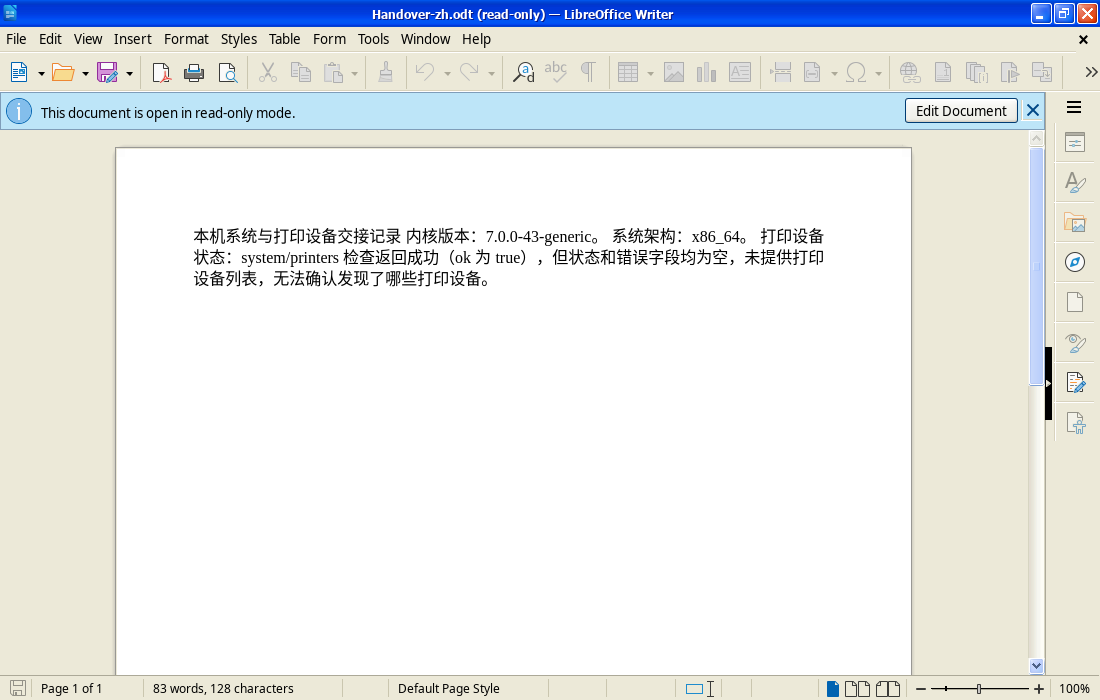
\includegraphics[width=.88\linewidth,height=75mm,keepaspectratio]{../assets/agent/laptop-20261125/writer-document-zh.png}\par
\small 笔记本实测：打开已生成的中文交接单。\end{center}
\section*{让 Agent 看懂当前窗口}
\sample{打开添加打印机向导，列出当前窗口名称和可以操作的控件，等我选择。}
助手可调用应用启动、窗口枚举和辅助功能查询。核对窗口后再要求下一步，例如“返回上一步”。可识别的控件取决于应用是否提供辅助功能信息。\href{https://bennix.github.io/AgentLinux/\#hardware-demo}{真机截图与可下载的示例文档}
\newpage
\chaptertitle{从本机终端调用组件}
在开始菜单打开“本机终端”。以下命令在已登录的 AgentLinux 桌面用户下运行。它们直接使用桌面助手的组件后端，适合脚本读取或排查模型返回的结果。
\section*{发现、查询、启动}
\begin{verbatim}
agentlinux-components --help
agentlinux-components
agentlinux-components system/printers
agentlinux-components --launch app/agentlinux-xp-add-printer.desktop
\end{verbatim}
第一条查看用法；第二条返回本机组件目录，其中 \texttt{system} 列出系统组件，\texttt{apps} 将应用 ID 对应到可读名称。第三条读取打印机状态。最后一条打开添加打印机向导；运行前可先在目录中核对该 ID。含空格的 ID 用引号括起。
\section*{怎样判断查询成功}
以下是没有配置打印队列时一台笔记本的实际返回：
\begin{verbatim}
{"component": "system/printers", "ok": true,
 "status": "", "error": ""}
\end{verbatim}
这里查询成功且状态文本为空。如果 \texttt{ok} 为假，查看 \texttt{error}。其他常用只读查询包括 \texttt{system/storage}、\texttt{system/power} 和 \texttt{system/network}。要启动 GUI 程序，请在目标图形会话内运行命令。
\section*{什么时候选哪个入口}
要让模型分步规划、读结果并继续追问，用桌面助手。已知组件 ID、需要可重复的查询时，用本机终端。要操作工作区并通过手机续接任务，用下一页的 ZenCode 工作台。默认隔离终端运行在 Cage 客机内；查询这台笔记本本身时，从菜单选择“本机终端”。
\newpage
\chaptertitle{通过微信续接 ZenCode 任务}
\begin{enumerate}
\item 从应用菜单打开 ZenCode，配置模型供应商，打开本次任务所用的工作区。先在桌面完成一个小任务，例如请它列出该工作区的文件。
\item 在工作台的“手机控制”中打开微信配对，用手机扫码，核对允许的账号和工作区。需要控制图形应用时，在 ZenCode 内启用电脑控制。
\item 保持该用户的图形会话及 ZenCode Host 运行。在手机上接着提问，例如“把刚才的文件清单整理成一份交接说明，保存到当前工作区”。收到权限请求时核对目标和操作，再作答。
\item 文件生成后，明确指定工作区内文件的名称，要求发送回当前微信会话。收到附件后打开核对版本和正文。
\end{enumerate}
\section*{遇到问题时}
\textbf{连接失败或提示模型不存在。} 核对供应商、Base URL 和完整模型 ID；确认密钥有权调用该模型，且当前网络可达所选接口。
\par\textbf{能聊天，但没有操作窗口。} 在桌面助手中检查“允许桌面操作”和模型工具调用能力；查看是否有待确认的对话框。用上一页的命令确认目标应用确实在本机目录中。
\par\textbf{要点的按钮找不到。} 先要求列出窗口，再查询目标窗口的控件。仍无对应项时，在桌面手动完成该步，再继续任务。
\par\textbf{手机没有收到文件。} 检查 Host 是否在线、配对账号和会话是否正确、文件是否位于已授权工作区，以及附件大小是否符合工作台提示。
\par\textbf{多步任务中途停下。} 先询问已完成的动作和文件路径，再只提交剩余步骤。重复创建或发送文件前先核对已有结果。
\vfill\href{https://bennix.github.io/AgentLinux/}{AgentLinux 产品页与版本下载}\hfill\href{https://github.com/bennix/AgentLinux}{项目仓库}

\newpage
\chaptertitle{用 Agent 操作 XP 资源管理器}
本页适用于已更新资源管理器的笔记本及候选镜像（SHA-256 前八位为 \texttt{643cae82}）。公开版 v2026.11.25.4 尚未包含本页所用的文件项接口。
\section*{准备一个练习目录}
在本机终端运行以下命令，再按 Win+R，输入下面第二行的命令打开资源管理器。示例中的目录名可自行替换。
\begin{verbatim}
mkdir -p "/tmp/AgentLinux Demo/Reports"
explorer.exe "/tmp/AgentLinux Demo"
\end{verbatim}
\section*{先选择，再确认，再打开}
\sample{在资源管理器的 AgentLinux Demo 窗口中找到 Reports 文件夹，选中它，读取选中状态，然后打开它。告诉我打开后的窗口标题。}
支持 AT-SPI 的桌面工具可以按以下顺序执行。若用 Python 编写 Agent，可通过系统 Python 的 \texttt{gi.repository.Atspi} 调用这些接口。
\begin{enumerate}
\item 从桌面辅助功能树找到应用 \texttt{explorer}，再找到标题为 \texttt{AgentLinux Demo} 的窗口。在该窗口内查找角色为 \texttt{LIST\_ITEM}、名称恰好为 \texttt{Reports} 的节点。
\item 在文件项上枚举动作名称，调用 \texttt{select}。读取状态集合中的 \texttt{SELECTED} 后，确认选中的是刚才的文件夹。
\item 调用同一文件项的 \texttt{open} 动作。重新读取窗口标题，应显示 \texttt{Reports}。也可读取地址栏，核对末尾的目录名。
\end{enumerate}
\section*{目录内容发生变化时}
用户删除文件或切换目录后，原来的文件项可能返回 \texttt{DEFUNCT}，可用动作数变为零。此时重新读取当前目录，按名称匹配目标，再核对选中状态。中英文界面使用相同的动作名称。

\end{document}
